%%%%%%%%%%%%%%%%%%%%%%%%%%%%%%%%%%%%%%%%%%%%%%%%%%%%%%%%%%%%%%%
%
% Welcome to Overleaf --- just edit your LaTeX on the left,
% and we'll compile it for you on the right. If you open the
% 'Share' menu, you can invite other users to edit at the same
% time. See www.overleaf.com/learn for more info. Enjoy!
%
%%%%%%%%%%%%%%%%%%%%%%%%%%%%%%%%%%%%%%%%%%%%%%%%%%%%%%%%%%%%%%%
%\usepgfplotslibrary{external}
%\tikzexternalize

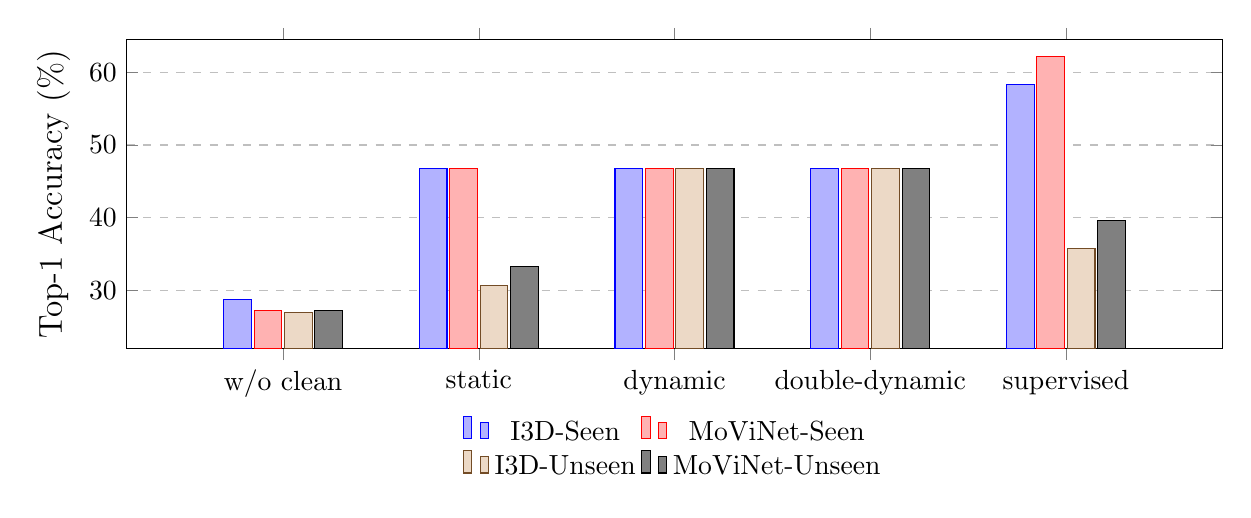
\begin{tikzpicture}
\centering
\begin{axis}[
symbolic x coords={w/o clean, static, dynamic, double-dynamic, supervised},
	ylabel=\large Top-1 Accuracy (\%),
	enlargelimits=false,
	ybar=1pt, enlarge x limits=0.2,
	xtick=data,
	ymin=22.0,
    ymax=64.5,
    ymajorgrids=true,
    legend style={draw=none},
          grid style=dashed,
          width=15.5cm,
          height=5.5cm,
         legend style={at={(0.5,-0.2)},
	    anchor=north,legend columns=2}, 
        every axis plot/.append 
        every mark/.append style={mark size=52pt}
]
\addplot 
	coordinates {(w/o clean,28.73) (static,46.77) (dynamic,46.77) (double-dynamic,46.77)
	(supervised,58.33) };
	\addlegendentry{I3D-Seen} 
\addplot 
	coordinates {(w/o clean,27.20) (static,46.71) (dynamic,46.71)(double-dynamic,46.77)
	(supervised,62.24) };
	\addlegendentry{MoViNet-Seen} 
\addplot 
	coordinates {(w/o clean,26.96) (static,30.71) (dynamic,46.71)(double-dynamic,46.77)
	(supervised,35.71) };
\addlegendentry{I3D-Unseen} 
\addplot 
	coordinates {(w/o clean,27.20) (static,33.30) (dynamic,46.71)(double-dynamic,46.77)
	(supervised,39.59) };
\addlegendentry{MoViNet-Unseen} 

\end{axis}
\end{tikzpicture}


